% Partie 1.2 - Les différents protocoles et topologies %

\subsection{Les différents protocoles et topologies}

\subsubsection{Les différentes topologies}

Un réseau local (\textbf{LAN} pour \textit{Local Area Network}) est un réseau où les terminaux peuvent communiquer sans avoir besoin d'un accès Internet. Mais il existe un autre type de réseau plus proche de nos contraintes, le réseau personnel (\textbf{PAN} pour \textit{Personal Area Network)}. Dans ce type de réseau le but est de faire aboutir les échanges entre les divers éléments du réseau avec des puissances assez faible pour garantir une autonomie correcte. Ce qui correspond bien à nos besoins avec les capteurs. Ils ont besoins d'être autonome le plus longtemps possible tout en évitant une interaction humaine physique direct. 

Dans le monde des réseau, nous utilisons le terme topologie pour définir l'arrangement des différents nœuds dans un réseau. Avec les réseaux PAN, on se limite assez souvent à deux topologies: maillage partielle (\textbf{mesh}) et en étoile (\textbf{star}).

La topologie en étoile est extrêmement rependue car c'est celle qui est utilisée dans le modèle maître-esclave(s). Le maître est le point névralgique du réseau, toutes les communications sont obligées de passer par lui. Cela se révèle assez pratique dans le cas de la collecte de données car le maître est le point de convergence en plus d'être le point de sortie du réseau.

Cette topologie est en parfaite opposition au maillage partielle. En effet dans cette dernière topologie chaque nœuds est potentiellement un routeur, et chaque routeur un potentiel point de sortie. Ces routeur sont appelés des \textit{Edge Router} ou \textit{Border Router}, ils font le lien entre le PAN et d'autres réseaux. Les End Devices ne routent pas l'information.

\begin{figure}[h]
\begin{center}
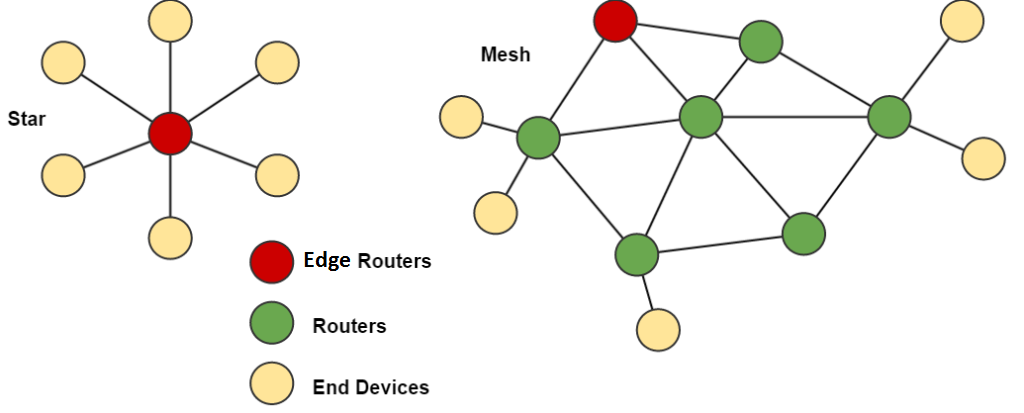
\includegraphics[width=15cm]{\rpDossier/images/topologies.png}
\end{center}
\caption{Topologies}
\label{topologies}
\end{figure}

Le fait est que comme cette technologie est explorée par plusieurs constructeur et organisme, plusieurs protocoles ont vu le jour, mais sans réel standard, chacun utilise celui qu'il veut. Cela pose pas mal de problème avec l'interopérabilité des éléments dans le réseau qui est pourtant une des caractéristiques phare de l'IoT. Voici une liste succincte de ces divers protocoles.

\subsubsection{les différents protocoles}

Dans cette partie nous allons vous présenter divers protocoles orientés basse consommation. Ces protocoles sont développées par divers organismes ce qui fait qu'aucun n'est un standard, les constructeurs implémentent ceux qui veulent. Cela peut poser certains problèmes d'interopérabilités, et augmenter fortement le prix des appareils.

\textbf{Zigbee} : 

\textbf{Bluetooth} :

\textbf{Wi-Fi} :

\textbf{Z-Wave} :

\textbf{IrDA} :